\subsection{General Molecular Dynamics Algorithm}

Starting with a given number of atoms $``N"$, one want to be able to simulate or predict how those atoms will be moving according to time. What will be the displacement or trajectory of these atoms at a different time. The algorithm works as follows:
\begin{enumerate}
    \item System Initial Configuration $\vec{r_{i}}(t=0)$ ; $\vec{v_{i}}(t=0)$\\
    Given a system of $``N"$ atoms, initial position vectors $\vec{r_i}$ and initial velocity vectors $\vec{v_i}$ at $t=0$, with $i=\{1,2,3,...,N\}$, are generated depending on the system configuration. In Section  \ref{subsec:about_} is explained how GROMOS software generates data sets for both initial position and initial velocities by minimisation and termalization processes respectively.
    \item Total Potential Energy $U_{ij}$ \\
    Given the initial configuration of the system, the inter-atomic potential energy between atoms now can be determined. Each pair of atoms potentially will have a given energy between them $U_{ij}$ because of the forces applied $\vec{F_{ij}}$. This interaction is determined by electrostatic (Equation \ref{eq:electrostatic}) and Van der Waals (Equation \ref{eq:LJ_pot}) forces and is intrinsically dependent on the distance between them $r_{ij}$. The total potential energy is equal to the sum of each pair interaction between atom $i$ and $j$.
    $$U_{tot}=\sum_{i\neq j}^N U_{ij}$$
    \item Determine Total Forces Applied\\
    With the potential energy $U_{ij}$ as a function of the distance $r_{ij}$ between two atoms, the force apply by a given atom $i$ on atom $j$ can be calculated by the gradient of the energy.
    $$ F_{i\rightarrow j}=-\vec{\triangledown } U_{ij}$$
    $$ \vec{F_i} = \sum_{i\neq j}^N F_{i\rightarrow j}$$
    Therefore, the resultant force on an atom $i$ must be the sum of all forces between it and all other atoms $j\neq i$. 
    \item Acceleration on each atom.\\
    Applying Newton's equations of motion and knowing the forces and the masses of each individual atom,  the acceleration applied on each atom is given by:
    $$\vec{a_i}=\frac{\vec{F_i}}{m_i}$$
    \item Prediction of Motion $r(t+dt)$ ; $v(t+dt)$\\
    Knowing the initial position and initial velocity of an atom $i$, and knowing it's acceleration one can predict how the atoms will be moving after a small increment of time $dt$. Now, one can calculate the new velocity $v(t+dt)$ and new position $r(t+dt)$ after a small increment in time. This relies on the numerical integration. Knowing the acceleration, it can be integrating in order to get the position and how the position is changing according to time. 
\end{enumerate}
Figure \ref{fig:md_algo} summarizes the algorithm described above. 
\begin{figure}[h]
    \centering
    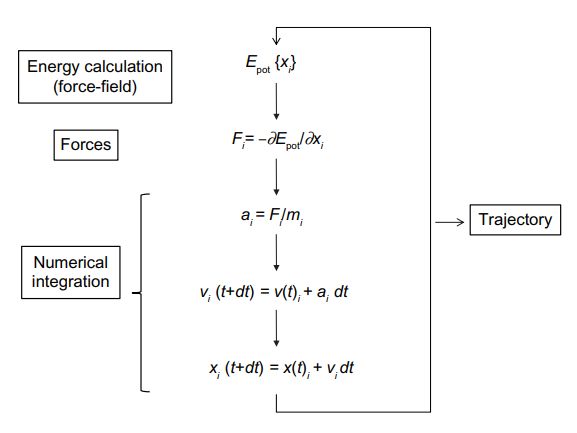
\includegraphics[scale=0.5]{Figures/Chapter2/md_algorithm.png}
    \caption{Molecular dynamics basic algorithm. Figure from Hospital \textit{et al.} \cite{hospital2015molecular}}
    \label{fig:md_algo}
\end{figure}

\subsubsection{Numerical Integration}\label{subsubsec:leapfrog}
Multiple methods to integrate equations of motion have been developed. Among these is the \textbf{leap-frog algorithm} \cite{leach2001molecular} which was used for the simulations carried out in this work. Figure \ref{fig:leapfrog} is a schematic representation of how the variables for velocities and positions are compute throw the mathematical scheme \cite{cuendet2007calculation}. 
\begin{figure}
    \centering
    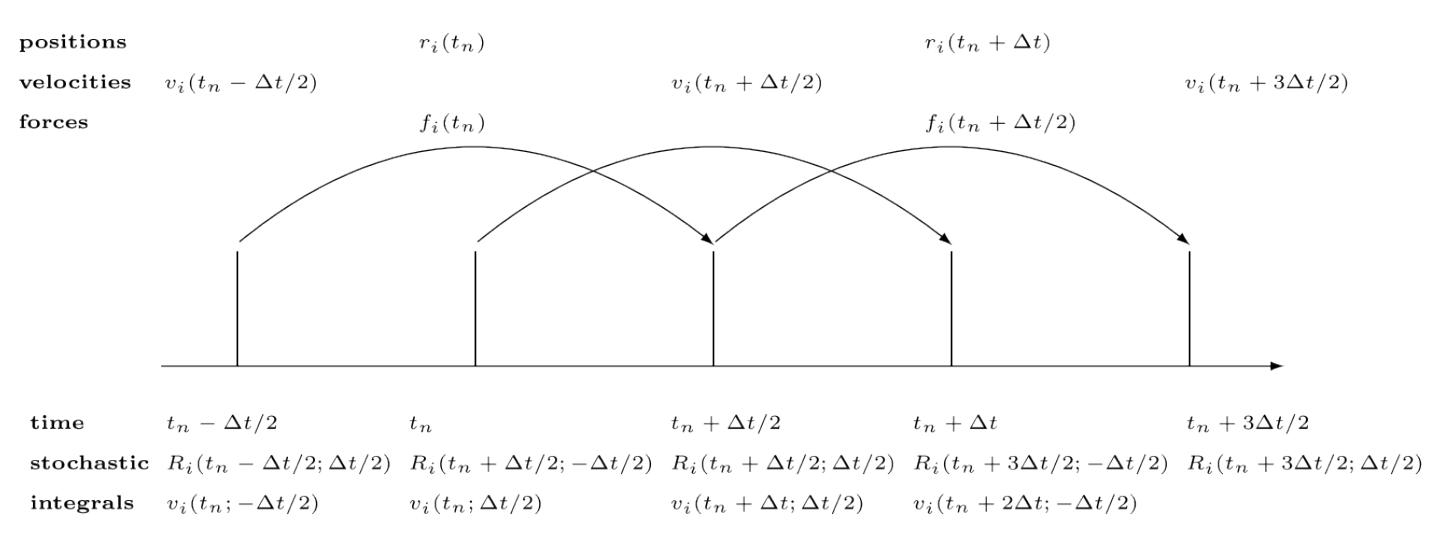
\includegraphics[scale=0.31]{Figures/Chapter2/Leap_Frog.png}
    \caption{The leap-frog integration scheme.Figure from Van Gunsteren: Gromos Manual Vol.2}
    \label{fig:leapfrog}
\end{figure}
When a Taylor expansion of the velocity $v_i(t_n-\Delta t/2)$ at $t=t_n$ is subtracted from
an expansion of $v_i(t_n+\Delta t/2)$ at $t=t_n$, neglecting terms of third and higher order for simplicity, results: 
\begin{equation}
    v_i(t_n+\Delta t/2) = v_i(t_n-\Delta t/2) + \frac{F_i(t_n)}{m_i}\Delta t
    \label{eq:v_i_tylor}
    \end{equation}
And similarly, when a Taylor expansion of the position $r_i(t_n)$ at $t=t_n + \Delta t/2$ is subtracted from an expansion of $r_i(t_n + \Delta t)$ at $t=t_n + \Delta t/2$ results (again neglecting terms of third and higher order for simplicity):
\begin{equation}
    r_i(t_n + \Delta t)=r_i(t_n) + v_i(t_n = \Delta t/2) \Delta t
    \label{eq:r_i_tylor}
\end{equation}
Equations \ref{eq:v_i_tylor} and \ref{eq:r_i_tylor} are the leap-frog velocity and position formulas, respectively, which together form the leap-frog scheme. This provides a simple method where a MD algorithm alternates between calculating (and updating) positions and velocities.

